%!TEX root = paper.tex
\clearpage
\appendix
\section{Process Management with Double-Fork}\label{app:doublefork}
\begin{figure}[H]\label{fig:process_sequence}
	\centering
	\begin{subfigure}{1.2\linewidth}
		\centering
		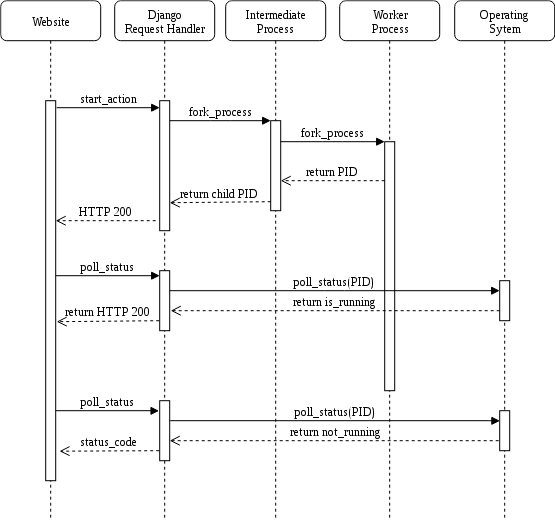
\includegraphics[width=1.5\linewidth]{figs/process_sequence}
	\end{subfigure}
	\caption{The sequence of internal requests to start a process and poll its status.}
\end{figure}

\clearpage
\section{Scenario-Based Testing}\label{app:scenariotest}
This appendix contains the test script for the scenario-based test cases as well as the reported results.
The below test cases reflect the flow from a user perspective starting from project setup and ending at the generated adversarial example.
Each test step defines a four-tuple of an action, an expected reaction, the actual reaction and whether the test is passed.
Please note that the software version under test is not the last commit on the master branch since we need perform the test and put the test results into the documentation.
The software is not affected by these changes and the test has been performed on January 15, 2019.
The commit hash is: c963c8c791eb2053d0cdd3cf4db27c0475711ee6 


\subsection{Test Case 1: Project Setup}
\begin{description}
	\item[Preconditions]: 
		\begin{itemize}
			\item [--] access to the git repository is granted or a snapshot of it is prevalent
			\item [--] the host machine runs a linux kernel
			\item [--] the host machine has docker installed
			\item [--] the host machine is connected to the internet
			\item [--] at least ca. 1 GB of memory
			\item [--] there is an empty directory read to be mounted as the data root into the docker container
		\end{itemize}
	\item[Test Steps]: 
	\begin{enumerate}
		\item  
		\begin{itemize}
			\item [-] open project's README and determine installation steps
			\item [-] the README contains a sequence of commands to run in order to create the docker container
			\item [-] there is a section called \enquote{setup} describing it
			\item [-] PASSED
		\end{itemize}
		\item  
		\begin{itemize}
			\item [-] create the docker image
			\item [-] the docker daemon returns no error message on exit
			\item [-] the docker daemon returns no error message on exit
			\item [-] PASSED
		\end{itemize}
		\item  
		\begin{itemize}
			\item [-] instantiate the docker container (first time, with empty data root mounted, with port 80 forwarded)
			\item [-] the setup script downloads the reference dataset, pip requirements and the web frameworks and performs Django migrations
			\item [-] the download commands complete without error and the Django migrations yield the output \enquote{OK}
			\item [-] PASSED
		\end{itemize}
		\item  
		\begin{itemize}
			\item [-] exit and instantiate the docker container again(second time, with filled data root mounted, with port 80 forwarded)
			\item [-] the setup script skips downloading everything except for the web frameworks and performs Django migrations
			\item [-] the download commands are skipped without error, the pip packages are installed from the local cache and the Django migrations yield the output \enquote{OK}
			\item [-] PASSED
		\end{itemize}
		\item  
		\begin{itemize}
			\item [-] open a web browser and visit localhost
			\item [-] the welcome page is shown, the standard output of the container shows some server output containing at least one HTTP 200 response and optionally some HTTP 302 responses
			\item [-] the welcome page is shown prompting for a valid api key, the standard output of the container shows one HTTP 200 response and multiple HTTP 304 (redirect) responses to GET requests for the JS and CSS frameworks
			\item [-] PASSED
		\end{itemize}
	\end{enumerate}
\end{description}

\subsection{Test Case 2: Model Training}
\begin{description}
	\item[Preconditions]: 
	\begin{itemize}
		\item [--] all requirements of test case 1 also apply here
		\item [--] a docker container as created by the test steps of test case 1 is running
		\item [--] the web browser is open and showing the welcome page on localhost, prompting for the api key
	\end{itemize}
	\item[Test Steps]: 
	\begin{enumerate}
		\item  
		\begin{itemize}
			\item [-] enter a random letter sequence and click on submit
			\item [-] the modal does not disappear and shows an error message
			\item [-] on entering \enquote{asdf} and submitting, the input field becomes red and a message is shown indicating that the key is invalid
			\item [-] PASSED
		\end{itemize}
		\item  
		\begin{itemize}
			\item [-] disable the host machine's network connection, reload the page and retry submitting
			\item [-] the modal does not disappear and shows an error message
			\item [-] on submitting, the input field becomes red after a few seconds and a message is shown indicating that the no connection to the remote server could be established
			\item [-] PASSED
		\end{itemize}
		\item
		\begin{itemize}
			\item [-] re-enable the host machine's network connection, reload the page and submit a valid key
			\item [-] the modal disappears and the welcome page is now in focus
			\item [-] on submitting, the modal disappears with an animation and the welcome page is now shown with focus
			\item [-] PASSED
		\end{itemize}
		\item
		\begin{itemize}
			\item [-] click on \enquote{models}
			\item [-] the models overview page is shown, indicating that there are no trained models yet
			\item [-] the models overview page is shown, indicating that there are no trained models yet
			\item [-] PASSED
		\end{itemize}
		\item
		\begin{itemize}
			\item [-] click on \enquote{Details} in the navigation bar
			\item [-] the model details page is shown, indicating that there is no running training process
			\item [-] the model details page is shown, indicating that there is no running training process
			\item [-] PASSED
		\end{itemize}
		\item
		\begin{itemize}
			\item [-] click on \enquote{Training} in the navigation bar
			\item [-] the page for starting a new training is shown
			\item [-] the page for starting a new training is shown
			\item [-] PASSED
		\end{itemize}
		\item
		\begin{itemize}
			\item [-] select rebuilding, a single training epoch, enter a model name and click on submit
			\item [-] on selecting rebuilding, further options appear; there are pre-filled default values for each parameter; submitting redirects to training details
			\item [-] on selecting rebuilding, further options appear; there are pre-filled default values for each parameter; submitting redirects to training details
			\item [-] PASSED
		\end{itemize}
		\item
		\begin{itemize}
			\item [-] navigate to training page and try starting a second training process
			\item [-] an error message appears and the training is not started
			\item [-] an error message appears and the training is not started
			\item [-] PASSED
		\end{itemize}
		\item
		\begin{itemize}
			\item [-] go back to the details page and reside there until the training has finished
			\item [-] the console window shows the output of the successful training; the abort training button disappears and is replaced by another button to clear the output
			\item [-] after ca. 3.5 minutes, the training has finished (with 79.98\% validation accuracy) which is shown in the console; the abort training button disappears and is replaced by another button to clear the output
			\item [-] PASSED
		\end{itemize}
		\item
		\begin{itemize}
			\item [-] navigate back to the overview page
			\item [-] the initial info disappeared and is replaced by a table containing one element with the name of the trained model
			\item [-] the initial info disappeared and is replaced by a table containing one element with the name of the trained model
			\item [-] PASSED
		\end{itemize}
		\item
		\begin{itemize}
			\item [-] click on the info icon
			\item [-] after a short loading animation, a table with the model's architecture is shown; it shall contain typical CNN layers like max pooling
			\item [-] after a short loading animation, a table appears containing entries like \enquote{conv2d} and \enquote{max\_pooling}
			\item [-] PASSED
		\end{itemize}
		\item
		\begin{itemize}
			\item [-] dismiss the modal, then train a second model as in the steps 6-7 (with a different model name)
			\item [-] a second model is successfully trained as tested before
			\item [-] a second model is successfully trained
			\item [-] PASSED
		\end{itemize}
		\item
		\begin{itemize}
			\item [-] navigate back to the overview
			\item [-] there are now two models in the table
			\item [-] there are now two models in the table
			\item [-] PASSED
		\end{itemize}
		\item
		\begin{itemize}
			\item [-] click on the trash can icon of the first model
			\item [-] a popover appears prompting to approve the action
			\item [-] a popover appears with the option to proceed (green) or cancel (red)
			\item [-] PASSED
		\end{itemize}
		\item
		\begin{itemize}
			\item [-] click on cancel
			\item [-] the popover disappears and nothing more happens
			\item [-] the popover disappears and nothing more happens
			\item [-] PASSED
		\end{itemize}
		\item
		\begin{itemize}
			\item [-] repeat step 14 but now click on \enquote{proceed} afterwards
			\item [-] the entry is deleted from the table, the table is updated without page reload
			\item [-] the entry is deleted from the table, the table is updated without page reload
			\item [-] PASSED
		\end{itemize}
		\item
		\begin{itemize}
			\item [-] click on the bolt icon on the remaining model
			\item [-] the browser is redirected to the attack page from where a new attack can be started
			\item [-] the browser is redirected to attack/attack.html, containing a form to submitting a new attack
			\item [-] PASSED
		\end{itemize}
	\end{enumerate}
\end{description}

\subsection{Test Case 3: Attack}
\begin{description}
	\item[Preconditions]: 
	\begin{itemize}
		\item [--] all requirements of test case 1 and 2 also apply here
		\item [--] the browser is open and is showing the welcome page after entering a valid api key
	\end{itemize}
	\item[Test Steps]: 
	\begin{enumerate}
		\item  
		\begin{itemize}
			\item [-] click on \enquote{attack}
			\item [-] the attack overview page is shown indicating that there are no attacks performed yet; there is a button redirecting to \enquote{Attack}
			\item [-] the attack overview page is shown indicating that there are no attack processes to be shown; there is a button \enquote{Go to Attack}
			\item [-] PASSED
		\end{itemize}
		\item  
		\begin{itemize}
			\item [-] click on \enquote{Go to Attack}
			\item [-] the attack starting page is shown; the only available model is preselected
			\item [-] the attack starting page is shown; the previously trained model is preselected
			\item [-] PASSED
		\end{itemize}
		\item  
		\begin{itemize}
			\item [-] choose an image file of size other than 64x64 pixels and submit the attack using the default parameters
			\item [-] an error message shows up
			\item [-] an error message shows up indicating the size mismatch: \enquote{was (1920, 1080) but expected (64, 64)}
			\item [-] PASSED
		\end{itemize}
		\item  
		\begin{itemize}
			\item [-] choose a valid image and submit the attack using the default parameters
			\item [-] the browser is redirected to the details page showing the attack progress in a console window; the source image is shown at the bottom together with the remote prediction
			\item [-] the browser is redirected to the details page showing the attack progress in a console window; the source image is shown at the bottom together with the remote prediction \enquote{Einmalige Vorfahrt}: 0.99161738
			\item [-] PASSED
		\end{itemize}
		\item  
		\begin{itemize}
			\item [-] wait until the attack has finished
			\item [-] the page now shows additional images including the adversarial example; there are remote predictions for each of them
			\item [-] the original image is shown again as well as the adversarial example; the remote prediction has been correct for the source image and shows the target class for the adversarial example
			\item [-] PASSED
		\end{itemize}
		\item  
		\begin{itemize}
			\item [-] navigate to attack overview
			\item [-] the overview includes an entry with a PID and some icons
			\item [-] the overview includes an entry with PID 198, \enquote{finished} badge and a trash icon
			\item [-] PASSED
		\end{itemize}
		\item
		\begin{itemize}
			\item [-] click on the PID
			\item [-] the same page like in step 5 is shown
			\item [-] the same page like in step 5 is shown
			\item [-] PASSED
		\end{itemize}
		\item
		\begin{itemize}
			\item [-] navigate back to attack overview; click on the trash icon
			\item [-] the table entry disappears; a message indicating that there are no attack processes appears
			\item [-] the table entry disappears and a message appears: \enquote{There are no attack processes to show at the moment.}
			\item [-] PASSED
		\end{itemize}
	\end{enumerate}
\end{description}